\chapter{Nonreentrancy and selective relinking: \\ the \textit{libgotcha} runtime}
\label{chap:libgotcha}

\ifdefined\chapquotes
\vspace{-1in}
\begin{chapquote}[1.5in]{James S.\@ A.\@ Corey, \textit{Nemesis Games}}
`Alien superweapons were used,' Alex said, walking into the room, \\
sleep-sweaty hair standing out from his skull in every direction. \\
`The laws of physics were altered, mistakes were made.'
\end{chapquote}
\fi

In Section~\ref{sec:libinger:reentrancy}, we saw that it is not safe in general for a
preemptible function to call into stateful code that was written without the
preemptible function abstraction in mind.  However, such code is prolific in the
modern systems stack, and in order to support interoperability with it, we need to
automatically transform the program to fix the safety hole.  This chapter introduces
a novel abstraction for memory isolation and constructs a software system that
implements it, dubbed \textit{libgotcha}; then, we conclude the chapter by presenting
performance metrics.

\begin{figure}
\begin{center}
\includegraphics[width=0.7\columnwidth]{figs/procimg_perobj}
\end{center}
\caption[Layout of a typical module within the process image]{
Layout of a typical module within the process image.  \textbf{Bold} sections
contain program data; \textit{italicized} ones contain metadata for the runtime.}
\label{fig:procimgobj}
\end{figure}

\begin{swallowsections}
\input[functions]{gotcha_gotcha}
\end{swallowsections}
\hspace{-1.5em}
Our discussion in this chapter uses \textit{libinger} as a motivating example of a
\textit{libgotcha} user, as this configuration was the inspiration for the runtime's
creation.  However, we have found the described techniques to be general and
equally relevant to applications beyond timed functions.  As such,
\textit{libgotcha} exposes a general API that allows any \textbf{control library} to
configure its behavior for the process.  We give more details later in the chapter,
and study other examples of control libraries in Chapter~\ref{chap:safety}.


\section{A brief tour of linking}
\label{sec:libgotcha:link}

We begin with background about linking, a two-stage process that ultimately produces
an in-memory \textbf{process image} containing a program's code, all the data it
needs to execute, and the code and data of all its dependencies.  Linking operates on
\textbf{object files} that can take the form of either an \textbf{executable} or a
\textbf{shared library}.  Once a program is running, its process image contains a
region corresponding to each loaded object file.  We will refer to each such region as
a \textbf{module}, regardless of whether it corresponds to an executable or a shared
library.  Each module is divided into logical \textbf{sections}, each containing a
particular type of information.  Figure~\ref{fig:procimgobj} shows a typical module's
layout; notice that it contains both data corresponding to the source code and
generated metadata for runtime consumption.

The linking process occurs in two parts.  Static linking occurs at compile time and
forms the last step of the traditional build process.  Dynamic linking occurs at a
phase of runtime known as \textbf{load time}, which starts before the
program has been loaded from disk or the language runtime initialized.


\subsection{Static linking}

Invoking the \texttt{cc} compiler driver does more than just compile C code:\@ it
runs the C preprocessor \texttt{cpp}, the C compiler (\texttt{cc1} in GCC's case),
then the static linker \texttt{ld}.

The output of the second step is a relocatable object file containing code and data
with referenced addresses identified by named \textbf{symbols}.  In a relocatable
object file, symbol \textbf{references} such as instructions making function calls
or accessing global variables are encoded with a null address as a placeholder.  Each
object file contains a \textbf{relocation table} in a separate section that
associates each placeholder with a symbol name, which may or may not be located in
the same file.  Each object file also contains a \textbf{symbol table} to identify
the symbols it defines and associate them with the file offset of their definition.
Note that only non-\texttt{static} C symbols generate global symbol table entries
that can be referenced from other object files; this keyword is confusingly named and
does not refer to static linking.  The compiler's ultimate output is one relocatable
object file for each source file.

The static linker is responsible for combining one or more relocatable object files
into a single executable or shared library, where either type of output file is
ready for loading into memory for execution.  This process consists of verifying that
there is a definition corresponding to each symbol reference, unifying the sections
across object files and choosing a final address (or relative address) for each
symbol, encoding the chosen addresses at the location recorded in each relocation
table entry, and writing the resulting file to disk.  This output file does not
preserve the relocation table because the linker has already fixed the null pointers
it described.  The file does contain a symbol table because it can be useful for
debugging (e.g., to generate stack traces), but this can be removed using the
\texttt{strip} utility without affecting the program semantics.

With the exception of macOS, most modern Unix systems use ELF (Executable and
Linkable Format) object files.  One advantage of this format is that executables and
shared libraries are themselves ELF object files.


\subsection{Dynamic linking}
\label{sec:libgotcha:dylink}
\label{sec:relinking}

Static linking allows programs to reuse ``libraries'' of precompiled object files,
but each program must be built with its own copy of all its libraries within the
executable.  This means that every time an application is loaded, its libraries' code
and data must be read back from disk, even if another running program uses the same
libraries; it also means that updating a library requires recompiling all dependent
programs installed on the system.  Dynamic linking solves both problems by separating
libraries into separate files that are not read until the executable runs.\footnote{
Specifically, this separation obviates the need to read the files from disk multiple
times because the runtime maps them into the process image using the \texttt{mmap()}
family of system calls.  The kernel tracks regions that are already mapped and serves
recurring requests from memory instead of disk, mapping to the same physical memory
if the pages are read-only or creating copy-on-write page mappings otherwise.}

By splitting libraries into their own files, dynamic linking introduces a build-time
challenge:\@ the relative position and offset of modules cannot be known until
runtime.  As such, rather than performing the relocations for inter-module symbol
references, the static linker leaves the placeholder addresses and adds a separate
dynamic relocation table and dynamic symbol table into the output object file.
Unlike the tables used for static linking, these are needed to launch the program, so
tools such as \texttt{strip} leave them in place.  For executables, the linker also
writes the path to an ``interpreter'' program into the ELF program header.

When asked to load a program that declares an interpreter, the kernel loads and jumps
to the interpreter instead of the executed program.  Usually, this interpreter is the
system \textbf{dynamic linker}, traditionally named \texttt{ld.so}.  Before jumping
into the program code, the dynamic linker loads all the modules and processes the
entries in each of their dynamic relocation tables.  The relocations are not
restricted to modifying writeable memory:\@ they can update constant global data and
even executable instructions.  Even if they leave the code unchanged, its position
relative to the rest of the module matters.  These points are critical to our use
case, as they mean that in order to duplicate modules' data, we must also duplicate
their code.

Another consequence of relocations being able to alter read-only memory is that the
dynamic linker must change the page protections of these regions after it has
finished
processing relocations.  To support this, the compiler splits up module components
into fine-grained sections by purpose.  Non-\texttt{const} global variables are
placed in the \texttt{.data} and \texttt{.bss} sections, which must remain writeable
at runtime and therefore require no special action.  In contrast, \texttt{const}
globals are split between the \texttt{.rodata} and \texttt{.data.rel.ro} sections
based on whether they require relocation; in the latter case, the dynamic linker
marks the pages read-only before passing control to the program.

If relocations routinely modified scattered locations throughout the executable
\texttt{.text} section, the dynamic linker would have to change page protections on
most or all of each module's code pages.  This would require a lot of system calls,
but it would also require copy-on-write code mappings, preventing instruction cache
hits between processes using the same library.  To avoid these problems, the compiler
indirects references to dynamic symbols via a structure called the GOT (Global Offset
Table).

\begin{figure*}
	\begin{minipage}{\textwidth}
	\includegraphics[width=\textwidth]{figs/gotables-crop}
	\subcaption{Reading a library's global variable: \texttt{size\_t tmp = data;}}
	\label{fig:dytabs:got}
	\end{minipage}

	\begin{minipage}{\textwidth}
	\includegraphics[width=\textwidth]{figs/pltables-crop}
	\subcaption{Calling an eagerly-resolved library function: \texttt{fun()}}
	\label{fig:dytabs:plt}
	\end{minipage}

	\begin{minipage}{\textwidth}
	\includegraphics[width=\textwidth]{figs/jstables-crop}
	\subcaption{Calling a lazily-resolved library function.  In step \textcircled{5},
	the dynamic linker memoizes the resolved address into the GOT; subsequent calls
	proceed as above.}
	\label{fig:dytabs:lazy}
	\end{minipage}
\caption[Table references required to reference global symbols]{
Table references required to reference global symbols in dynamically-linked
programs}
\label{fig:dytabs}
\end{figure*}

The GOT is a table of relocated pointers to symbol definitions, whether those
definitions are within the same module or in a different one.  To avoid generating
code pages that require relocations, the compiler compiles each reference to or
dereference of non-\texttt{static} global data into a position-independent load of
the corresponding pointer from the GOT.  Figure~\ref{fig:dytabs:got} shows an example
of the two instructions and one table reference needed for a dereference.  A
reference would generate only the first \texttt{mov} instruction, as would taking a
pointer to a function.

Calling a global function works differently and relies on another indirection
structure called the PLT (Procedure Linkage Table), which contains code instead of
pointers.  For each call to a non-\texttt{static} function, the compiler generates a
position-independent call to a PLT entry corresponding to the function being called.
It generates a PLT entry, which is a short sequence of instructions that loads the
pointer to the real definition from the GOT, then executes an indirect jump to that
location.  Figure~\ref{fig:dytabs:plt} shows an example function call.  As with GOT
entries, there are PLT entries for functions defined both within and outside the
referencing module.

Not all function calls are this simple.  To save the dynamic linker some work at load
time, many function calls resolve lazily on their first execution.  Such resolution
involves a series of jumps designed to memoize the address so that subsequent calls
to the function from the same module do not repeat the expensive lookup.
Figure~\ref{fig:dytabs:lazy} shows the effect of the first call to such a
function:\footnote{This representation is slightly simplified for brevity.  In
practice, it is undesirable to hardcode the address of a dynamic linker function into
each module.  Therefore, instead of jumping directly to the symbol resolver, the slow
lookup path jumps to a dedicated PLT stub that loads its address from another GOT
entry.  Technically, there are separate identifiers for the symbol and the module,
each pushed to the stack by one of these two involved PLT stubs.}
\textcircled{1}~The
program calls the PLT stub, just as it would for an eagerly-resolved function.
\textcircled{2}~The PLT stub is longer (three instructions instead of one), but still
begins with an indirect jump to the pointer found in the corresponding GOT entry.
\textcircled{3}~The GOT entry initially contains the address of the PLT stub's second
instruction, so the indirect jump is a no-op and merely advances the instruction
pointer.  \textcircled{4}~The rest of the PLT stub pushes a constant identifying the
module and symbol onto the stack, then jumps to a symbol-lookup function in the
dynamic linker.  \textcircled{5}~After looking up the address of the symbol's
definition, the dynamic linker uses the identifier from the stack to find and update
the GOT entry in the calling module.  \textcircled{6}~The dynamic linker jumps to the
symbol in the defining module.  Because the GOT entry has been updated, future calls
proceed exactly like eagerly-resolved ones and jump directly to the symbol definition
from the first instruction of the PLT stub.  Of course, the GOT entries associated
with lazy PLT stubs must be writeable at runtime; this is why
Figure~\ref{fig:procimgobj} shows the GOT as split between two sections.

The dynamic linker performs all relocations and other standard module setup
automatically at load time, but the initialization process is pluggable.  In
particular, modules can include \textbf{constructor} functions to be invoked before
control is transferred to the runtime and ultimately the program's main function.  As
we will see, our work leverages this feature to override certain relocations at the
conclusion of load time.


\begin{promotesubsections}
\input[functions]{gotcha_namespaces}


\input[functions]{gotcha_libsets}
\end{promotesubsections}

Thus, selective relinking is selective in two ways, only affecting execution when the
next libset differs from the current libset and the program references a dynamic
symbol defined in a module that is not currently executing on that thread.


\subsection{Detecting cross-module symbol references}
\label{sec:libgotcha:crossref}

Identifying which GOT entries correspond to cross-module symbol references is a
multi-step process:
First, we traverse the relocation table for each loaded module, cross referencing
each of its relocation entries against the local module's symbol table.  If the
symbol table does not contain a definition matching the relocation entry's target, we
conclude that the relocation must correspond to a cross-module call.  Otherwise, we
check the address in the GOT entry corresponding to the relocation:  If this address
is outside the memory bounds of the current module, it is a cross-module call.
Otherwise, if this address matches the one from the symbol table entry, it is not a
cross-module call, and should be skipped.  The trickiest case is when the GOT entry
does not match but does point somewhere within the current module, since this means
it probably still refers to the PLT stub (because the symbol reference is lazy and
has not yet been resolved, as covered at the end of
Section~\ref{sec:libgotcha:dylink}).  In this case, we resolve the symbol early,
update the GOT entry, and recheck whether it resolved to the local definition to
determine whether it is a cross-module call.


\begin{promotesubsections}
\input[functions]{gotcha_init}
\end{promotesubsections}

If a preemptible function is \cancel{ed} rather than being allowed to return,
execution might be interrupted within a call to a library function.  For this reason,
\textit{libgotcha} must treat the libset's shared state as corrupted; it provides the
\texttt{libset\_reinit()} function shown in Listing~\ref{lst:gotchaapi} to allow
control libraries to inform it of such a situation so it can \textbf{reinitialize}
the libset before returning it to the pool.

Our early approach to reinitialization was to unload and reload all objects in the
libset by calling \texttt{dlclose()} followed by \texttt{dlmopen()}.  While this
approach theoretically allowed us to delegate the work to the dynamic linker, in
practice it introduced significant complications.\footnote{Most notably, some shared
libraries are marked with a special configuration flag, \texttt{DF\_1\_NODELETE},
which prevents the dynamic linker from ever removing them once they have been loaded.
Because almost all libraries depend on libc, the presence of even one such library
would prevent us from reinitializing a libset.  The flag is mostly used on libraries
that need to monkey-patch some other loaded library, such that the two subsequently
have a circular dependency.  Fortunately, this was not generally a problem for us
because when we unload one library from a libset, we then unload the rest.  Whenever
we encountered a \texttt{NODELETE} object file, we would make a special copy with the
flag cleared, for loading into every namespace except the main one.}  Worse, it
required the dynamic linker to reprocess all relocations throughout the libset, which
introduced prohibitive runtime latency.  We measured reinitialization taking almost 5
ms (over 10 million cycles on modern processors) on even minimal example
programs~\cite{boucher:atc2020}.  With such delays, the only reasonable way for the
control library to handle cancellation was to delegate the reinitialization to a
separate thread to take it off the critical path; of course, this approach only works
as long as the number of libsets is not a bottleneck.

We have since redesigned reinitialization around a significantly faster approach:\@
checkpointing only portions of each module.  The key insight is that, as we saw in
Section~\ref{sec:libgotcha:link}, only some sections are writeable at runtime.  We
can therefore assume that these are the only memory regions of each module that can
change.  After populating the libset pool at application start, \textit{libgotcha}
iterates through each module of each libset and makes a backup copy of all its
writeable regions.  When a control library calls \texttt{libset\_reinit()},
\textit{libgotcha} restores each such region from the backup before returning the
affected libset to the pool.  We summarize this approach, which reduces the
latency of reinitialization by two orders of magnitude, in
Figure~\ref{fig:reinit}.\footnote{We will address the version watermark alluded to
therein later in this chapter.}  To avoid having to repeat relocations and rerun
module constructors, we capture the backup after dynamic relocation is complete and
all constructors have run; the tradeoff is that we must actually copy memory,
rather than leveraging copy on write to later restore to the version on disk.

\begin{figure}
\includegraphics[width=\columnwidth]{figs/reinit-crop}
\caption{Libset reinitialization to support asynchronous cancellation}
\label{fig:reinit}
\end{figure}


\section{Selective relinking}
\label{sec:libgotcha:relink}

Most of the complexity of \textit{libgotcha} lies in the implementation of selective
relinking, the mechanism underlying libset switches.  To establish the libset
abstraction, it must arrange to conditionally intercept cross-module symbol
uses based on the currently-configured next libset.

As we saw in Section~\ref{sec:libgotcha:dylink}, whenever a program references a
dynamic symbol, it looks up the address of the definition in a data structure called
the global offset table (GOT).  Selective relinking works by shadowing the
GOT.\footnote{Hence the name \textit{lib\textbf{got}cha}.}  Just after the dynamic
linker populates the GOTs, \textit{libgotcha} replaces every entry that should
sometimes trigger a libset switch with a fake address.  It stores the original
address in its shadow GOT, which is organized by the libset that houses the
definition.  The fake address used depends upon the type of symbol:


\subsection{Intercepting function calls}
\label{sec:libgotcha:functions}

When setting up selective relinking, we do not know whether a particular function
call needs to be rerouted until runtime.  However, the fact that dynamic function
calls consult the GOT to determine which code to execute makes it efficient and
relatively straightforward to receive a notification whenever they occur.  To set
this up, at load time, we replace each such cross-module GOT entry with the address
of the special \textit{libgotcha} function \texttt{procedure\_linkage\_override()}.
Whenever the program tries to call one of the affected functions, control transfers
to this function instead; it then checks the thread's next libset, looks up the
appropriate symbol definition in the shadow GOT, and jumps to that location.  Because
\texttt{procedure\_linkage\_override()} runs between the caller's \texttt{call}
instruction and the real function, it is written in assembly to avoid clobbering
registers (e.g., those used for argument passing).

There is one major complication that necessitates an additional level of indirection
beyond what we have described.  Recall from the eagerly-resolved function calling
sequence in Figure~\ref{fig:dytabs:plt} that each function call site calls a
one-instruction PLT stub that performs an indirect jump to the real definition via
the GOT.  This means that if we simply replaced all the GOT entries with the address
of \texttt{procedure\_linkage\_override()}, that function would not know which GOT
entry it was being called via, and therefore which symbol to look up.  Instead, we
introduce our own table of executable stubs called the PLOT (Procedure Linkage
Override Table).  Unlike PLT entries, ours always push an identifier indicating which
function is being called.  For this, we use indices into a custom data structure
called the GOOT (Global Offset Override Table), which stores enough information to
find the symbol's shadow GOT entries while being practical to traverse in handwritten
assembly code.  Figure~\ref{fig:override} summarizes the modified dynamic function
call sequence under selective relinking.

\begin{figure}
\includegraphics[width=\textwidth]{figs/tables-crop}
\caption{Calling an eagerly-resolved library function under selective relinking}
\label{fig:override}
\end{figure}

A subtle but important point about dynamic linking is that pointers to the same
definition must compare equal, regardless of where they are obtained.
The reader might notice that invocation is not the only thing a program can do with a
function:\@ it might also pass around the function's address.  In fact, after taking
the address, it could pass it to code within a different module, which might need to
know whether a third module passed a pointer to the same function.  To support such
comparisons, the compiler exclusively generates eagerly-resolved relocations for any
function that a particular module obtains a pointer to.  This way, the \texttt{mov}
to retrieve the pointer always finds the resolved address of the real definition in
the GOT.  To avoid breaking pointer comparison, \textit{libgotcha} allocates a single
PLOT entry for each function definition, rather than using a separate one for each
call site or dependent module.  This
provides correct comparison semantics because all references to a particular function
receive the same pointer to the shared PLOT entry, and although this pointer
technically refers to the corresponding symbol's definitions in all libsets, at any
one time all calls to it will only resolve to the definition in the next libset.
Since at any given time there can only be one next libset, calls to pointers that
compare equal always refer to the same copy of the definition.

The setup described so far works for eagerly-resolved function calls.  However,
recall that some function calls resolve to their definition lazily at runtime.  For
such calls, the dynamic linker memoizes the resolved address by updating the GOT
entry, as shown in Figure~\ref{fig:dytabs:lazy}.  Unfortunately, replacing this GOT
entry would overwrite the PLOT pointer installed by \textit{libgotcha} at load time,
thereby preventing it from intercepting future calls to the function.  The write to
the GOT happens within the symbol-lookup code in the dynamic linker, so there is no
way to skip it.  Luckily, the dynamic linker keeps each module's dynamic relocation
table in memory and uses that to determine which GOT entry to update.  The
\textit{libgotcha} constructor exploits this by marking the relocation table pages
writeable, changing the relocation entries corresponding to cross-module calls, then
restoring the protection bits.  This fools the dynamic linker's lazy symbol lookup
into later updating the shadow GOT entry instead.  Not only does this avoid breaking
selective relinking, it also preserves memoization.

The GNU system supports a second, nonstandard type of lazy function call resolution
known as indirect function calls.  Compared to the lazy resolution specified in the
ELF standard, this variant allows the defining library to provide custom code to
resolve the address of the function definition.  We must support this mechanism
because glibc relies on it to select among architecture-specific implementations for
reasons of optimization (e.g., \texttt{strstr()}, which leverages vector extensions
on processors that have them) or simply portability (e.g., \texttt{clock\_gettime()},
which depends on the best available time source).  Indirect symbols require special
handling because their definitions are misleading:\@ the symbol table entry in the
defining module describes the location not of the definition but of a function that
returns that definition's location.  If we placed such addresses into our shadow
GOTs, each caller would unwittingly invoke the resolver function instead of the
function it was trying to call.  Whenever we see a symbol table entry marked with the
\texttt{STT\_GNU\_IFUNC} type, we instead invoke it and place the returned pointer in
the shadow GOT.  A final complication is that some indirect resolver functions
retrieve their return values from the GOT, so if we call them after we have
manipulated it, they can create inefficient chains of calls through multiple shadowed
GOT entries, or even infinite recursion where a resolver returns the PLOT stub that
leads to the very shadow GOT entry it was intended for.  To avoid these problems, we
call all of a module's indirect resolvers eagerly and save the results into the
shadow GOTs before making any changes to the real GOT.


\subsection{Intercepting global variable accesses}
\label{sec:libgotcha:globals}

Unlike function calls, global variable accesses do not provide an opportunity for
hijacking the flow of control to detect the dereference, so we rely on operating
system assistance to implement a mechanism similar to demand paging.  At load time,
we replace each cross-module global variable GOT entry with a carefully-chosen
address within a mapped but inaccessible memory region.  The program is therefore
able to retrieve a ``pointer to'' the global variable, but whenever it attempts to
read from or write to the location, it generates a segmentation fault;
\textit{libgotcha} registers a signal handler so such signals notify it rather than
crashing the program.  The handler disassembles the faulting instruction to determine
the base address register of its address calculation and attempts to reconstruct a
GOOT pointer based on the invalid address in that register.  If successful, it checks
the thread's next libset, retrieves the address of that libset's definition of the
symbol from the appropriate shadow GOT, and replaces the base address register's
contents with this address.  It then returns, causing the processor to reexecute the
faulting instruction with the valid address this time.  From the application's
perspective, it is as if dereferencing the phony pointer causes it to change into a
real address.  To avoid breaking applications with their own segmentation fault
handlers, \textit{libgotcha} intercepts calls to \texttt{sigaction()} and keeps a
pointer to the third-party handler.  Whenever its handler is unable to resolve a
segmentation fault, it forwards the signal to the third-party one.

The above approach assumes that the program will read or write from the global
variable, but the global variable could instead contain a function pointer.  If it
does and the program tries to invoke it, it will use an indirect call instruction and
the jump will succeed but transfer control to an invalid location.  In this
situation, it is important that we do not attempt to disassemble the faulting
instruction, as the instruction pointer is pointing to unreadable memory.  However,
we can recognize this case because the address of the fault matches the instruction
pointer itself (instead of whatever address the instruction would have been trying to
load data from).  To find the indirect call instruction, we load the return address
from the stack; this gives us the subsequent instruction, so we subtract the length
of an indirect call instruction.  We alter the signal handler's context so that the
operating system will transfer control back to this instruction when our handler
returns, then we disassemble the instruction and follow our usual approach on its
register operand.

It is possible to generate other code sequences that are incompatible with the
approach (e.g., because they perform in-place pointer arithmetic rather than using a
displacement-mode address calculation with a base address), so we also employ a few
heuristics that consider the context of the instruction and fault.  If the code is
reading or writing to a faulting location that we cannot translate into a GOOT
pointer, it might have applied a linear offset to the last address we successfully
translated.  If any of the following indicators point to this, we compute the offset
between the faulting address and the last invalid address we replaced, then compute
the replacement register value by adding this offset to the last replacement address
we substituted:

\begin{itemize}
\item The client code is using the same base address register as it was when
	we last intercepted a global variable access.  This might indicate that
	said code is using the register as an address accumulator, but doing
	so in concert with some other temporary register: because of this
	indirection, overwriting the register with the temporary after we
	had preformed the original address resolution would have left us
	unable to process any subsequent values accumulated into the register.
\item The base address register is different than the one updated on our last
	interception, but the value of the latter has
	remained unchanged since we updated it.  Because it contains a memory
	address we had to resolve, this strongly suggests that the client code
	has only executed a few instructions since then, which we can infer
	even if that set included one or more branch instructions.
\item The current return address points to the instruction immediately
	following the one that last faulted,
	and the current base address register's value has
	remained the same since the faulting instruction was executed.  This
	implies that said instruction was an indirect procedure call, and that
	the register was probably just used to pass a pointer argument.
	Because we didn't resolve the address of the indirect call until the
	client code was already transferring control, there was no way for it
	to have passed a pointer without performing arithmetic directly on the
	dummy address present before the call.
\end{itemize}

In our experience, these heuristics cover the common cases in compiler-generated
code.  We do not allow heuristics to chain (that is, we never use a
heuristically-calculated address as the basis of the offset calculation for another),
but we do apply heuristics multiple times based on the same base address.

While our current approach has proven successful, it does have some downsides.  It is
complex, relies on heuristics, and incurs a performance cost on the order of
microseconds.  It also suffers from a design flaw affecting large structures:\@ it
does not account for the size of globals when ``allocating'' them fake addresses
within the inaccessible memory region.  If a fake address gets assigned to a global
whose size is less than the difference between that address and the end of the
inaccessible region, it is possible for a correct program to dereference outside the
inaccessible region and exhibit emergent undefined behavior.  The ELF dynamic symbol
table includes objects' sizes, so it would be possible to account for this when
assigning fake addresses.

One could go further with this idea and redesign global variable interception without
the need for heuristics or the dependency on a disassembler.  By allocating each
global its own inaccessible region matching its real size, the address of the
faulting access could be made to reveal the access's offset within the global.
Mapping the fake address back to a symbol would require a lookup data structure; one
option is a hash table with an entry for each of our inaccessible pages.  To
translate a fake address, one would zero out its page offset bits, consult the lookup
structure to find our metadata about the page, and use this to convert to a real
symbol definition and offset within it.  This final conversion could be done either
by starting each global's fake region on a page boundary (at the cost of more virtual
memory) or binary searching a list of the addresses within the inaccessible page that
corresponded to the starts of new symbols\footnote{The faulting address would not be
found if the program was dereferencing at an offset into the global, but one would
just return the next-lowest entry.} (at the cost of logarithmic worst-case lookups
instead of constant average-case ones).


\section{Uninterruptible functions}
\label{sec:libgotcha:unint}

Unlike prior work, we support safe asynchronous pausing and cancellation on almost
any instruction boundary, including within most third-party libraries without
the need for configuration or code annotation.  However, there are still some cases
where we must briefly defer preemption.

The most obvious is the \texttt{malloc()} family of dynamic memory allocation
functions.  This case is significant because the allocator manages the heap, a
resource shared among all threads of the application.  As we saw in
Section~\ref{sec:functions:motivation}, na\"ive attempts to provide asynchronous
cancellation
often corrupt the heap if they interrupt the allocator.  It is even unsafe to
call into the allocator from a thread that has only been asynchronously paused while
allocating, as it can cause a deadlock on the locks intended to protect the heap from
concurrent access by different threads.  This is the reason why signal handlers are
not allowed to allocate memory.  One way around these problems would be to use a
separate heap for each preemptible function, but we have avoided this because it
would complicate the ownership of objects that are allocated by a preemptible
function but escape its scope before it terminates.

Instead, we consider the interfaces to the dynamic allocator to be
\textbf{uninterruptible} functions.  Although each libset contains a separate copy of
them, all except one are inactive.  Specifically, we route all calls to
uninterruptible functions back to the \textbf{starting libset}, the set of modules
loaded before \textit{libgotcha} loaded any additional copies.  The set of
uninterruptible functions is currently governed by an internal allowlist within
\textit{libgotcha}.  During load time, the constructor transcribes this information
into the shadow GOTs so lookups will incur no additional runtime overhead.

\begin{sloppypar}
Although the next libset does not determine which copy of an uninterruptible function
gets invoked, it is relevant during the call.  To avoid creating a dependency between
the starting libset and the current one, it is important that the next libset be set
to the starting libset while any uninterruptible code is running.  To preserve
this invariant, whenever \texttt{procedure\_linkage\_override()} detects that any
libset other than the starting one is calling an uninterruptible function, it resets
the next
libset to the starting libset, storing a backup of the previous value.  Then, just
before invoking the function, it pushes the address of a trampoline function onto the
stack.  When the function eventually returns, this trampoline runs; before
transferring control back to the call site, it restores the next libset.
\end{sloppypar}

In addition to controlling \textit{libgotcha}'s treatment of calls to uninterruptible
functions, the next libset also communicates valuable information to the control
library.  The starting libset must always be valid, and because we maintain the
invariant that the next libset is always equal to the starting libset when the
current libset is and third-party code is executing,\footnote{By third-party code, we
mean code that does not interact with the selective relinking primitive or any
abstraction built on top of it.  Any code that makes use of selective relinking is
responsible for doing so safely (i.e., ensuring that it does not corrupt its own
state).} it is safe to preempt execution if and only if the next libset
is not equal to the starting one.  It is crucial that the control library check this
before deciding to preempt, and as we saw in Listing~\ref{lst:gotchaapi}, it can do
so using the \texttt{libset\_thread\_get\_next()} function.

Unlike function calls, accesses to global variables do not have defined end points
after which they are complete.  That is, a single write might leave a structure in a
temporarily-invalid state that is corrected by a subsequent one, but there is no
structural association between the two.  We do not currently change the next libset
when we resolve a global variable access, which means a control library might pause
or cancel code in the middle of such a write or sequence of writes.  This is safe
because the allowlist does not contain any writeable variables, so the only time that
a global variable write can resolve to a definition in a different libset is when the
current libset is the starting one, the next libset is any other one, and the program
performs an access such as (1) from Listing~\ref{lst:exmplstate}.  Such an access
would be routed to the code's own libset, so any corruption due to concurrency would
remain properly isolated and could not infect the starting libset.\footnote{If one
did need support for allowlisted writeable global variables, the resolver signal
handler described in Section~\ref{sec:libgotcha:globals} would need to serve a
read-only copy of such variables; this way, each write would generate an additional
segmentation fault and the handler could batch writes to the backing object.
Determining a safe boundary for this batching would require at least additional
runtime heuristics, if not static analysis.}


\subsection{Other uninterruptible functions}
\label{sec:libgotcha:unintfuns}

The memory allocator interfaces are not the only functions in the allowlist.  The
dynamic linker behaves specially with respect to namespaces:\@ although it appears to
be loaded into every namespace, it refuses to load additional copies of itself and
instead includes special logic that proxies calls to it from other namespaces back to
the main one.  If such calls were considered interruptible, the proxying would
change the current libset out from under \textit{libgotcha}, violating the invariant
that the next libset must equal the starting libset when the current one does and
potentially corrupting the dynamic linker.  To
avoid this, we add all of the dynamic linker's functions to the allowlist.

The dynamic linker introduces other complications as well.  While itself dependency
free, the GNU implementation is part of the glibc project, and other glibc modules
depend on it, including on internal interfaces that should not be exposed to the rest
of the program.  To keep these interfaces private, the dynamic linker does not export
them as dynamic symbols, and instead exposes them via an opaque data region whose
layout is partially known to the other glibc modules.  Fortunately, the region is
split into separate subregions under the \texttt{\_rtld\_global\_ro} and
\texttt{\_rtld\_global} dynamic symbols based on whether the area is writeable, which
helps us determine whether a particular use has the potential to corrupt the dynamic
linker state.  In particular, we have allowlisted all the functions that access the
latter structure, a set currently consisting of \texttt{fork()},
\texttt{posix\_spawn()}, \texttt{uselocale()}, and
\texttt{\_\_cxa\_thread\_atexit\_impl()} from \texttt{libc.so} and
\texttt{pthread\_create()} from \texttt{libpthread.so}.  To flag potential breakage
from future changes in the region's use, \textit{libgotcha} emits a warning at load
time whenever it encounters an unexpected access to \texttt{\_rtld\_global}.

We have encountered one instance where a glibc module modifies
\texttt{\_rtld\_global} without a corresponding dynamic function call.  The
libpthread constructor monkey patches the dynamic linker to replace pointers to
stubbed-out mutex functions with its own proper implementation before the application
can spawn any POSIX threads.\footnote{It also installs hooks to support stack
execution protection and enable full support for thread-local variables.  As with the
mutex changes, these tweaks appear to replace stubbed placeholders rather than
establish information flow from the dynamic linker to the specific copy of
libpthread.}  These changes would create a hazardous dependency between the dynamic
linker and whichever copy of libpthread was last loaded (in our case, the one in the
last libset).  To avoid this problem, \textit{libgotcha}'s constructor checks for
libraries that (1)~directly access \texttt{\_rtld\_global}, (2)~have the type of
constructor in question, and (3)~are marked with the ELF configuration flag
\texttt{DF\_1\_NODELETE} to indicate that they are unsafe to unload once present in
the process image.  Before loading copies of a library with all of these properties
into any libsets, we create a temporary copy of its shared library with its ELF
metadata tweaked to prevent the constructor from running.  We add these patched
libraries to the beginning of the search path so libsets do not modify the dynamic
linker at load time and it continues to depend on the copy of libpthread in the
starting libset.

In a few places, a glibc module asks the dynamic linker to load or unload another
shared library at runtime by calling the internal \texttt{\_dl\_open()} or
\texttt{\_dl\_close()} interface using a function pointer hidden in
\texttt{\_rtld\_global\_ro}.  The most obvious of these is the public-facing
functions in \texttt{libdl.so}, the same interface that \textit{libgotcha} uses to
populate libsets.  We considered adding all of this library's functions to the
allowlist, but this presents a problem:\@ in order to decide which namespace to load
the library into, \texttt{dlopen()} checks which module contains its return
address.\footnote{Note that this means a \texttt{dlopen()} loads the module into the
current libset rather than the next one.  We preserve this standard system behavior
even though it is somewhat surprising.  The only time it could cause unexpected
results is when a module containing a preemptible function definition loads other
modules at runtime, and since it used preemptible functions, such a module could be
expected to be aware of this case.  If this choice later proved problematic to
application designers (e.g., of systems that make heavy use of runtime plugins), it
would be possible to instead base the destination on the next libset by injecting a
trampoline return address from the appropriate copy of \textit{libgotcha}.}
Treating it as uninterruptible would result in a libset switch when calling it from
outside the starting libset, pushing a \textit{libgotcha} trampoline ``return''
address onto the stack and thereby causing all dynamically-loaded libraries to be
added to the starting libset instead of the current libset.  Other functions that
use these internal dynamic loading calls include the \texttt{iconv()} family of
character-conversion functions, \texttt{getaddrinfo()} and the other DNS-translation
functions (which can load GNU Libidn to handle internationalized domain names), and
the modular Name Service Switch system for accessing the users, hosts, protocols,
and services databases.  Adding these functions to the allowlist would not break
them, but it would treat what are potentially long-running operations (even including
network communication) as uninterruptible code.  We instead handle both of these
situations by
replacing the \texttt{\_dl\_open()} and \texttt{\_dl\_close()} pointers in
\texttt{\_rtld\_global\_ro} with our own hook functions that transition to
uninterruptible code only while modules are being loaded or unloaded.  Since the
region is opaque and its layout is subject to change and dependent on the glibc build
configuration, we find the appropriate
pointers by repeatedly replacing one entry at a time with a probe function and
executing no-op
\texttt{dlopen()} and \texttt{dlclose()} operations until the probe function gets
called.  Once we have found both pointers, we record their original values, mark
their containing page writeable, replace them with pointers to our hook functions,
and restore the page protections.
\\


\subsection{Control library callbacks}
\label{sec:libgotcha:callbacks}

\begin{figure}
\begin{lstlisting}[label=lst:gotchacbapi,caption=\textit{libgotcha} C callback interface]
// Pointer to function taking and returning void
typedef void (*libset_cb_t)(void);

void libset_register_callback(libset_cb_t);
void libset_register_returnback(libset_cb_t);
libset_t libset_of_caller(void);
\end{lstlisting}
\end{figure}

While a control library can identify an uninterruptible task by observing that the
thread's next libset is equal to the starting one, many control libraries will
benefit from active notification of interruptibility.  For this purpose,
\textit{libgotcha} provides
a callback interface that allows the control library to register functions that
should be invoked whenever an uninterruptible function is called or returns.  A
control library can use such \textbf{call callbacks} and \textbf{return callbacks}
to disable and reenable preemption mechanisms or establish a critical
section around uninterruptible code (e.g., by taking a mutex or blocking signals).
Callbacks run when we automatically switch to the starting libset from any other;
since this change is idempotent, a callback is only invoked once at the beginning or
end of each uninterruptible region, even if the function calls others within the
starting libset.  Figure~\ref{fig:gotchahooks} shows the effect of such callbacks on
function call interception by comparing against both interruptible calls and
uninterruptible calls when no callbacks are registered.

\begin{figure*}
	\begin{minipage}{\textwidth}
	\includegraphics[width=\textwidth]{figs/calltree_function-crop}
	\subcaption{Interruptible call}
	\end{minipage}

	\begin{minipage}{\textwidth}
	\includegraphics[width=\textwidth]{figs/calltree_function_switch-crop}
	\subcaption{Uninterruptible call when no callbacks are registered}
	\end{minipage}

	\begin{minipage}{\textwidth}
	\includegraphics[width=\textwidth]{figs/calltree_function_hook-crop}
	\subcaption{Uninterruptible call when callbacks are registered for both calls and returns}
	\end{minipage}
\caption[Interception of cross-module function calls]{
Interception of cross-module function calls. Solid lines represent function calls;
dashed ones represent returns. Color marks uninterruptible code (i.e., next libset =
starting libset).}
\label{fig:gotchahooks}
\end{figure*}

Listing~\ref{lst:gotchacbapi} shows the functions for managing callbacks, which form
an extension to the main \textit{libgotcha} control API.  The control library can
pass a function pointer to either of the registration functions to have it invoked on
entry to or exit from uninterruptible code.  In developing this interface, we
discovered it was very hard to write correct callbacks that could tolerate being
preempted, so we elected to run all callbacks with the next libset set to the
starting one.\footnote{This is actually only currently true of the call callback, as
return callbacks run in the caller's libset for largely historical reasons.  We
originally made this decision because this callback type predated the mechanism for
querying the caller's libset.  After adding both this feature and call callbacks, we
planned to change the behavior for consistency between the two callback types, but
encountered a complication.  Some publicly-callable and initially uninterruptible
\textit{libgotcha} functions sometimes need to change the next libset partway through
in order to finish in an interruptible state, and we did not want such changes to be
observable by the callback.}
Recall that it is never safe to pause or cancel execution in this
state, so the control library's preemption mechanism will defer preemption in
callbacks, just as it was already required to do in other such places.  Because the
control library's callback might want to know which libset control switched from, we
provide a \texttt{libset\_of\_caller()} function for retrieving the previous value of
the next libset (which is also the value it will be restored to when exiting the
uninterruptible region).

\begin{sloppypar}
The way that we currently implement callbacks places some restrictions on what they
are allowed to do.  The \textit{libgotcha} assembly trampoline that invokes return
callbacks backs up the integer return registers, but such callbacks cannot use
floating point unless they manually save and restore the floating-point return
registers.  As an implementation shortcut, \texttt{procedure\_linkage\_override()}
invokes the call callback via a \texttt{SIGTRAP} handler by executing an
\texttt{int3} instruction, in order to avoid having to save and restore a large set
of registers itself (since the return registers account for only two of the many
caller-saved registers).  The signal occurs at a well-known point in execution (e.g.,
not in the middle of memory allocation), so it does not subject the callback function
to the usual safety constraints on signal handlers, but it does make this type of
callback orders of magnitude slower.  Fortunately, we anticipate rarer need for them;
\textit{libinger}, for example, only uses a return callback.
\end{sloppypar}


\section{Control libraries}
\label{sec:libgotcha:control}

Selective relinking is a low-level abstraction useful in
special situations that require fine-grained memory isolation (e.g., legalizing types
of concurrency that would otherwise exhibit undefined behavior).
As such, \textit{libgotcha} takes no stance on
how libsets should be applied, instead leaving it up to other code to use them (by
changing the next libset).  We refer to this other code as a control library because
it controls \textit{libgotcha} using the API shown in Listings~\ref{lst:gotchaapi}
and \ref{lst:gotchacbapi}.

The semantics of a control library depend on how it is built:
\begin{itemize}
\item An \textbf{internal} control library is statically linked with
	\textit{libgotcha} to form a single shared object file that is loaded (or
	preloaded) as one unit.  Because each libset contains a separate copy of
	its module, \textit{libgotcha} adds itself to the uninterruptible allowlist
	described in Section~\ref{sec:libgotcha:unint}.  This redirects all calls to
	it into the starting libset, rendering its other copies dormant in a manner
	similar to the dynamic linker's proxying mechanism.  By virtue of being part
	of \textit{libgotcha}'s module, internal control libraries enjoy the same
	guarantee that their code always executes in the base libset.\footnote{There
	is actually one exception to this rule:\@ control libraries written in Rust
	can include generic functions in their public interface.  Because rustc
	monomorphizes such functions for the client code that uses them,
	\textit{their implementations are not actually in \textrm{libgotcha}'s
	module!}  Rather, there are one or more copies of them (specialized for
	various type arguments) in each program module that calls them.  It is
	difficult to write correct control library code that can tolerate preempting
	itself or interacting with other copies of itself, so we recommend that
	control libraries with generic interfaces manually transfer control to the
	starting libset before doing the bulk of their work.  One way to improve the
	experience for control library authors would be to provide a procedural macro
	compiler plugin that would at least partially automate this using custom Rust
	attributes.}  This also means that
	they, like \textit{libgotcha}, are automatically considered uninterruptible.
\item An \textbf{external} control library is dynamically linked with
	\textit{libgotcha}, and therefore constitutes a separate shared object file
	that depends on \texttt{libgotcha.so} (or, perhaps, a compatible internal
	control library).  Calls into such a library do not cause an automatic libset
	switch unless explicitly allowlisted within \textit{libgotcha}, so the
	library is responsible for coping with preemption and multiple copies of
	itself.  Despite these limitations, support for external control libraries
	enables control libraries to compose without mutual build system support,
	allows a single application to have more than one unrelated control library,
	and supports updating to a new version of \textit{libgotcha} without
	rebuilding the control library.
\end{itemize}


\subsection{Enforced interposition}
\label{sec:libgotcha:interpose}

A few libc functions either present an opportunity to circumvent the libset
abstraction or misbehave when called from a program that uses libsets.  To address
this, \textit{libgotcha} uses a dynamic-linking trick called \textbf{interposition}
to substitute its own implementation of these functions.  Interposition occurs when
one module defines a symbol with the same name as another module's symbol, resulting
in calls intended for the other module being routed to it instead.  This relies on
the interposing library appearing earlier in the dynamic linker's dependency search
order, so the technique is only reliable when the application binary is the
interposer or the interposing library is preloaded by defining the
\texttt{LD\_PRELOAD} environment variable before executing the application.

While \textit{libgotcha} supports being preloaded, it is intended to work seamlessly
even when the application is launched normally, so normal interposition is not strong
enough.  Fortunately, we already control dynamic linking by rewriting GOT entries, so
at the same time, we implement a variant that we term \textbf{enforced
interposition}.  Whenever we encounter a relocation in a third-party module
referencing a dynamic symbol with the same name as one defined in
\textit{libgotcha}'s module, we replace its GOT entry with the address of the PLOT
stub corresponding to that definition, so that all calls to that symbol from any
other module are redirected to \textit{libgotcha}.\footnote{We export a minimal and
deliberate subset of \textit{libgotcha}'s functions as dynamic symbols to avoid
unexpected applications of this rule.}  Conversely, whenever we encounter such a
dynamic symbol that is also referenced from \textit{libgotcha}'s module, we replace
its GOT entry there with a reference to the real third-party definition (or
interposition, as the case may be).  In this way, the code in \textit{libgotcha} can
implement wrappers around standard library (or any other) functions without
inadvertently interposing its own uses thereof.

We saw in Section~\ref{sec:libgotcha:globals} that one fraught case is the
\texttt{sigaction()} function, which could be used to replace the \textit{libgotcha}
signal handler that resolves global variable accesses at runtime to the appropriate
definition under the rules of selective relinking.  As such, we provide a replacement
implementation that checks whether the caller is trying to install a \texttt{SIGSEGV}
handler; if so, instead of honoring the request, we store the handler internally and
our handler calls it whenever it is unable to recover from a segmentation fault by
fixing one of our fake addresses.  We provide a similar replacement for the legacy
\texttt{signal()} function.  One other signal-related problem can occur when an
application or library temporarily blocks signals to establish a critical section.
Blocking our handler would cause the critical section to crash if it accessed a
global variable, so we replace \texttt{sigprocmask()} and \texttt{pthread\_sigmask()}
to leave \texttt{SIGSEGV} alone.  Finally, we replace \texttt{sigfillset()} and
\texttt{sigaddset()} to exclude \texttt{SIGSEGV}, which prevents signal handlers from
implicitly masking and unmasking it (via Linux's \texttt{sigreturn()} helper
function\footnote{This function is provided by the kernel for direct use by
unprivileged code.  It is defined in the VDSO (Virtual Dynamic Shared Object), an
emulated shared library that the kernel maps into each processes's address space.}).
The latter replacements are simple enough
to make good examples, so we include them in Listing~\ref{lst:gotcharepl}.  Note that
although they may appear recursive, they are not:\@ enforced interposition rebinds
their references to their own names to the external definitions in \texttt{libc.so}.

\begin{figure}
\begin{lstlisting}[label=lst:gotcharepl,caption=\textit{libgotcha} \texttt{sigfillset()} and \texttt{sigaddset()} replacements]
int sigfillset(sigset_t *set) {
	int res = sigfillset(set);
	if(!config_noglobals())
		sigdelset(set, SIGSEGV);
	return res;
}

int sigaddset(sigset_t *set, int signum) {
	if(!config_noglobals() && signum == SIGSEGV)
		return 0;
	return sigaddset(set, signum);
}
\end{lstlisting}
\end{figure}

Another troublesome call is \texttt{dlsym()}, used to manually look up the address of
a dynamic symbol by name.  For the same reason we encountered with \texttt{dlopen()}
in Section~\ref{sec:libgotcha:unintfuns}, simply marking it as uninterruptible would
cause it to search the wrong libset.  Because it implements its logic directly in
\texttt{libdl.so} rather than deferring to a private dynamic linker interface, we
initially assumed it would work fine out of the box; however, when we implemented the
warning about direct accesses to \texttt{\_rtld\_global} described in that section,
we were surprised to find that \texttt{dlsym()} triggered it.  Some investigating
revealed that \texttt{dlsym()} was directly taking the dynamic linker's big lock for 
the entire duration of every lookup because, whenever it hands one module the address
of a symbol defined in another, it adds a dependency edge between them to ensure the
defining module cannot be unloaded before the referencing one.\footnote{Technically,
there is one other reason for taking the big lock:\@ to prevent a concurrent
\texttt{dlclose()} from removing the defining module and/or corrupting the dependency
graph while the symbol search is in progress.  Unloading modules is a rare operation
that we currently consider out of scope, so we do not guard against this situation.
However, one feasible approach would be to replace \texttt{dlclose()} with a version
that took a \textit{libgotcha}-local lock to establish mutual exclusion with symbol
lookups without taking the big lock.  To avoid making symbol lookups uninterruptible,
\texttt{libset\_reinit()} could break the local lock in response to cancellation.  A
simpler option would be a \texttt{dlclose()} replacement that disallowed unloading
modules from libsets other than the starting one; this would have the additional
benefit of preventing a preemptible function from making a lasting change to the
modules available in its (reusable) libset.}  To solve this and prevent many manual
symbol lookups from being uninterruptible, we implemented a \texttt{dlsym()}
replacement that becomes interruptible (by restoring the next libset) and does not
take the big lock when it detects that the calling code's current libset is not the
starting one and that it is looking up a symbol in some specific other module in that
libset.  This is safe because such lookups can only modify the dynamic linker state
corresponding to their own libset, and the state changes (or any breakage caused by
pausing or cancellation) will therefore not impact any other libsets.\footnote{We
currently remain interruptible if it is traversing the entire global search list
rather than searching a specific module, because the symbol might resolve to a
definition in the dynamic linker.  In this case, the dynamic linker would add a
dependency edge into the starting libset because of the dynamic linker's special
proxying.  We suspect that such searches could safely be made preemptible if one
checked the symbol being searched against the dynamic linker's symbol table to ensure
this outcome was impossible.}  Our replacement function also makes one important
tweak to the symbol lookup semantics:\@ if we have a PLOT entry or fake global
address for the requested symbol, we return that instead of its true definition to
avoid creating a backdoor around selective relinking and to preserve pointer
comparison.  As part of these changes, we also had to add a
\texttt{dlerror()} replacement to report errors encountered during symbol lookups.

Finally, we encountered one apparent incompatibility between exception handling and
dynamic linker namespaces.  After noticing that Rust panics would crash the program
when the current libset was not the starting one, we discovered that libgcc and
libunwind's implementations of the \texttt{\_Unwind\_RaiseException()} function from
the C++ ABI (Application Binary Interface) call glibc's \texttt{dl\_iterate\_phdr()}
function to find each module's
\texttt{.eh\_frame} section containing metadata about the stack frame address.  We
then noticed that the latter function only searches the invoking namespace, which
causes unwinding to fail as soon as it encounters a function call that crossed a
namespace boundary.  We fixed this by adding a replacement implementation that
extends the search to other namespaces as long it has not yet found the module the
caller is seeking.

Because internal control libraries are within the same module as \textit{libgotcha},
enforced interposition treats them in the same special way.  This enables such
control libraries to define their own replacements merely by implementing a function
with a well-known name and exporting it in their dynamic symbol table.  By default,
all of their own uses of such a symbol refer to the third-party definition.  We
recognize that control libraries may need to further wrap our replacement functions
instead of overriding them completely, however, so for each symbol
\texttt{\textit{name}} that \textit{libgotcha} implements a replacement for, it also
exports a symbol \texttt{libgotcha\_\textit{name}} that refers unambiguously to that
replacement.  These symbols are local by default to prevent abuse, but any control
library that needs them can configure its build system to change their type before
linking against the \textit{libgotcha} static library.


\subsection{Thread-local storage}
\label{sec:libgotcha:tls}

Selective relinking seeks to isolate global state that would otherwise infect the
entire program if left corrupted or inconsistent by pausing or cancellation.  We saw
in Section~\ref{sec:libgotcha:relink} that this state includes global variables and
functions (which might be nonreentrant).  However, there is a third class of state
that escapes a function's scope:\@ thread-local variables.

Thread-local variables reside in a memory region known as the TLS (Thread-Local
Storage).  This, in turn, is located just before the TCB (Thread-Control Block), a
region storing metadata about the thread (Figure~\ref{fig:procimgthd}).  The pthreads
implementation maintains a pointer to the current thread's TCB in the \texttt{\%fs}
segment register for fast access, so the compiler simply translates references to
thread-local variables into negative offsets into that segment.\footnote{This is a
slight simplification because the layout of the TLS depends on the order in which
libraries are loaded, and therefore is not fully known until \textit{runtime}.
Depending on the thread-local variable's scope and which module it is defined in, the
dynamic linker may have to determine the offset in the middle of program execution.
Each combination of these two factors constitutes a different access ``model,'' and
causes the compiler to emit a different sequence of instructions to find the
variable.}

Unlike the types of state we have seen so far, the desired semantics of thread-local
variable accesses depend on how the control library is using libsets.  For some use
cases, it may even be necessary to widen the scope of thread-locals \textit{beyond
their thread}; for instance, this is required to support pausing code on one kernel
thread and then resuming its execution on a different one.  Furthermore, there is no
efficient way to consistently make relinking selective based on the module
relationship between the referee and the referent because TLS pointer calculations do
not use GOT entries and can use hardcoded offsets.  But neither is it clear whether
the abstraction provided by any given control library can tolerate a thread-local
variable's apparent value changing as soon as the next libset does and while the
current libset remains the same, which would make \texttt{thread\_local} variables
fail assertions analogous to (2) and (3) from Listing~\ref{lst:exmplstate}.

Rather than being opinionated and choosing the wrong stance, \textit{libgotcha}
defaults to the system behavior, where thread-local variables are
associated with the thread and unaffected by the next libset (though of course they
do depend on the current libset, since the TLS contains a separate copy of each
thread local for each copy of its defining module).  However, it anticipates that the
control library might want to maintain multiple sets of ``thread''-local variables by
allocating custom TCBs and swapping their pointers into the segment register.  One
hazard for this approach is that \texttt{pthread\_self()} simply retrieves the TCB
pointer from the thread segment register, so changing it alters the thread's view of
its own identifier.  The most significant consequence of this is that if the thread
attempts to send itself a signal (e.g., to support preemption), the thread ID it
passes will be invalid and the operation will fail.  To address this, we provide
replacement functions for the \texttt{arch\_prctl()} function for updating segment
registers\footnote{Although x86-64 processors provide an instruction for updating the
segment registers, the operating system can disable its use by non-supervisor code.
The Linux kernel does so to guard against a class of privilege-escalation bugs, and
instead provides a system call for changing segment registers so that it can validate
the new location before applying the update.  While a rogue application could avoid
our replacement function by calling \texttt{syscall()} instead of the glibc wrapper
function, this is a rare case and a difficult one to guard against.} and the
\texttt{pthread\_kill()} function for sending signals directed at a specific thread.
Respectively, our replacements store the pointer to the original TCB the installed
one is replacing and substitute the original pointer when they see one saved.

\begin{figure}
\includegraphics[width=\columnwidth]{figs/procimg_perthd}
\caption{Per-thread portion of process image}
\label{fig:procimgthd}
\end{figure}

One thing that \textit{libgotcha} does have to do is restore the TLS upon a
cancellation, since failing to do so might leave it permanently corrupt.  A na\"ive
approach would be to do this for every thread's TLS, but this could be quite
expensive, especially since it would require thread synchronization.  Instead, we
observe that each libset is likely to only ever be used by a single thread, and that
threads that never use a particular libset will never reference their TLS areas that
correspond to it.  Consequently, we reinitialize TLSes lazily:
We allocate a thread-local variable (per TCB, of course) to track each TLS's current
``version'' of each libset.  Whenever a control library calls
\texttt{libset\_reinit()} to signal a cancellation, we merely increment a separate
program-wide version watermark for that libset, as shown at the bottom of
Figure~\ref{fig:reinit}.  We know that a libset whose execution has just been
\cancel{ed} cannot currently be in use by any thread, so we do not need to do
anything
further unless and until the libset is reused.  We can recognize such reuse because
it begins with the control library passing the libset identifier to
\texttt{libset\_thread\_set\_next()}, and we respond by checking the current TCB's
current version for that library against the watermark.  If the TCB is out of date,
we iterate over the TLS's regions and restore the contents corresponding to modules
from that libset using each module's initialization image in its \texttt{.tdata}
and \texttt{.tbss} sections.  Then we update the TCB's current version for that
libset to match the watermark.  Of course, the control library might have multiple
TCBs that it uses with the same libset, but we detect this by following the same
procedure from our \texttt{arch\_prctl()} replacement function.
Figure~\ref{fig:tlsreinit} summarizes the algorithm; note that it is even robust to
control libraries that use the same libset from multiple threads concurrently, as
long as they never illegally reinitialize a libset while it is in use by any thread.

\begin{figure}
\includegraphics[width=\columnwidth]{figs/reinit_tls-crop}
\caption{Lazy TLS reinitialization following asynchronous cancellation and libset reuse}
\label{fig:tlsreinit}
\end{figure}

It is important that if a control library switches the TCB, it does not affect
\textit{libgotcha}'s internal state.  Yet \textit{libgotcha} relies on thread-local
variables to store information such as the pointer to the thread's original TCB.  In
addition to the enforced dynamic interposition mechanism described in the previous
section, \textit{libgotcha} includes a static interposition system whereby it can
define statically-linked replacement functions (not exported to the dynamic symbol
table) that apply throughout its own code but not to the rest of the program, even
internal control libraries.  This works because the static linker prefers to link
against static symbols provided directly in object files so that it can avoid
generating relocations against the GOT, but given the choice between (static) symbols
in a static library and (dynamic) ones in a shared library, it prefers to link
against the latter (so for internal control libraries, the third-party definition
rather than \textit{libgotcha}'s static replacement).  To insulate its own
thread-local variables against TCB changes, \textit{libgotcha} includes a static
replacement for the dynamic linker's \texttt{\_\_tls\_get\_addr()} function that
reroutes all its accesses to its own thread locals to the original TCB for the
current thread.\footnote{There are currently three thread locals that
\textit{libgotcha} deliberately accesses via static offsets from the TCB instead of
using \texttt{\_\_tls\_get\_addr()}.  The first stores the current version counters
for each libset, and is truly specific to the TCB rather than the kernel thread.  The
other two still correspond to the kernel thread, but are accessed from assembly by
\texttt{procedure\_linkage\_override()} and its return trampoline, whose
implementation is greatly simplified by being able to access them without calling
into C code.  One is the thread's record of the next libset before the libset switch,
which our \texttt{arch\_prctl()} replacement manually copies over whenever the
control library swaps in a different TCB.  The other is the actual next libset, which
is always set to the starting libset while a TCB swap occurs because of said
function replacement, and the trampoline will automatically restore its value from
the aforementioned upon return from the uninterruptible call.}


\section{Limitations}

Selective relinking successfully mitigates the shared state problem to allow safe
forms of asynchronous pausing and cancellation on top of the existing systems stack.
That said, we should emphasize a few shortcomings of our approach:


\subsection{Portability}
\label{sec:libgotcha:portability}

Selective relinking is grounded in general principles of dynamic linking and the ELF
specification.  The main burden of porting \textit{libgotcha} to another architecture
would be rewriting the assembly portions (\texttt{procedure\_linkage\_override()},
its trampolines, and the PLOT stubs), which currently account for under 300 lines of
code.  However, porting to another operating system would be more difficult, as
selective relinking requires linker namespaces, which are only available natively on
Solaris derivatives and the GNU system (although modern versions of Android's Bionic
runtime appear to include internal dynamic linker features sufficient to support the
namespace abstraction~\cite{www-bionic-bypass}).  And of course, selective relinking
is only relevant to dynamically-linked applications, which precludes its use in
embedded systems or with those programming languages that do not bother to support
dynamic linking.

Furthermore, getting \textit{libgotcha} to run real unmodified applications has
required handling many GNU/Linux-specific features and behaviors.  Examples include
indirect function calls (Section~\ref{sec:libgotcha:functions}); dynamic linker
proxying, glibc-wide shared state, monkey patching, and implicit module loading
(Section~\ref{sec:libgotcha:unintfuns}); \texttt{sigreturn()} signal masking, big
locks that escape the dynamic linker, and the interaction between namespaces and
exception handling (Section~\ref{sec:libgotcha:interpose}); and thread-local storage
details such as TCB switching and \texttt{\_\_tls\_get\_addr()}'s interface
(Section~\ref{sec:libgotcha:tls}).  As such, porting to a different dynamic linker
and C library would surely require a fair amount of systems hacking and debugging.

Indeed, \textit{libgotcha}'s degree of dependence on glibc means that even upgrades
can require some
work.  We originally developed \textit{libgotcha} atop glibc 2.29, and we found that
both the 2.30 and 2.31 releases introduced breaking changes.\footnote{The 2.30
release stopped accepting position-independent executables as arguments to the
\texttt{dlopen()} family of functions because they can contain \texttt{COPY}
relocations that break if they are not present from the start of the program.  As we
discuss later in this section, we do not support such relocations anyway.  However,
we need to open a copy of the executable in each libset just like any other module,
so we work around the change by stripping the \texttt{DF\_1\_PIE} ELF flag from the
executable using the same approach we use for monkey-patching constructors
(Section~\ref{sec:libgotcha:unintfuns}).  The 2.31 release introduced a dependency
between the number of supported namespaces and the size of the
\texttt{\_rtld\_global\_ro} structure.  At hundreds of libsets, this caused the
member to grow as large as 16 pages, triggering the symbol size limitation discussed
at the end of Section~\ref{sec:libgotcha:globals}.  We responded by increasing the
(currently hardcoded) number of inaccessible pages used to intercept global variable
accesses.}  Fortunately, we have prioritized debuggability throughout the development
of \textit{libgotcha}, and provide several features to make it less painful.  Among
these are a shell script for tracing intercepted function calls and global variable
accesses, a GDB script that automatically loads debugging symbols for namespaces
other than the starting one, environment variables for disabling features that make
debugging difficult (e.g., global variable interception, which generates numerous
segmentation faults), and specific workarounds to support running under
Valgrind~\cite{seward:usenix2005} and Mozilla's rr reverse
debugger~\cite{callahan:arxiv2017}.  With the help of these tools, we were able to
port to both glibc versions; furthermore, \textit{libgotcha} subsequently survived
the 2.32 and 2.33 upgrades unmodified.\footnote{More recently, glibc 2.34 has
consolidated the interfaces formerly exposed by \texttt{libpthread.so} and other
files into a monolithic \texttt{libc.so}.  As of this writing, we have not tried to
run \textit{libgotcha} atop this version, but we expect this major restructuring to
require at least minor changes.  We suspect the problem is not unique to us:  In the
more than six months since the upstream release, most major GNU/Linux distributions
have not yet stabilized this version.  This includes distributions such as Arch and
Gentoo that are typically known for shipping bleeding-edge packages.}


\subsection{Scalability}
\label{sec:libgotcha:scalability}

Although \textit{libgotcha} is compatible with an unmodified glibc in principle,
vanilla glibc builds are limited to 16 dynamic linker namespaces including the main
one.  This means that we can only create up to 15 new libsets, and that a control
library can only have this many preemptible tasks running and/or paused at any time.
To raise this limit, we rebuild the glibc sources with an increased value of
the \texttt{DL\_NNS} macro, which controls the number of supported namespaces.  There
is no need to install the resulting runtime on the host system; instead, we supply a
custom interpreter path when linking any application that needs more libsets.  We
have tested this configuration up to 512 namespaces, but the setting remains a fixed
(glibc)
compile-time limit.  Removing the per-process libset limit altogether would require
porting \textit{libgotcha} to work with an alternate dynamic linker that allocates
namespaces at runtime, such as drow~\cite{www-drow-loader}.

Relatedly, \textit{libgotcha} itself prepares all libsets at load time, and therefore
delays program startup in proportion to both the number of libsets and the number of
modules.  The good news is that doing this work up front significantly reduces the
latency at runtime.  That said, initializing libsets at runtime would allow control
libraries to strike their own balance between startup time and runtime cost.
Selective relinking is not fundamentally incompatible with such a feature, but
supporting it would require significant engineering effort, most notably modification
of all existing data structures to support resizing.

Initializing more than a few libsets reveals another scaling limitation in glibc:\@
certain dynamic libraries include eager relocations that require their thread-local
variables to be assigned TLS offsets at load time.  To support this, the GNU dynamic
linker reserves a certain amount of static TLS space that must be sufficient for all
libraries with this requirement across all namespaces.  Populating the libsets
multiplies modules' space requirements, and can quickly exhaust this static area.
Part of the problem is that \textit{libgotcha} itself includes such relocations to
make its assembly portions easier to write, and since it currently loads copies of
itself into each libset, it too contributes to the increased footprint.  When
launching a program
that must support more than a few libsets, one must export an environment variable
to tune glibc's static TLS size.


\subsection{Flexibility}
\label{sec:limits}

Selective relinking supports all but one of the cross-module dynamic relocation
types.  All forms of \texttt{GLOB\_DAT} relocations work:\@ global variables,
eagerly-resolved function calls, and indirect function calls.  Lazily-resolved
function calls via \texttt{JUMP\_SLOT} relocations work as usual (including
memoization), except that we must eagerly resolve some of them to determine
whether they represent cross-module calls.

All TLS access modes are supported by swapping out the TCB, although the semantics of
thread-local accesses depend on the control library's choice of when to do so.
Unlike with global relocations, selective relinking does not reroute cross-module
accesses based on the next libset, so the control library has the choice between
resolving all thread-local variable accesses to their definition in either the
current libset or the next libset at any given time.  While either of these choices
might be confusing, thread-local ``globals'' are quite rare.  Of the three such
variables remaining in glibc's \texttt{libc.so}, only \texttt{errno} was ever part of
its stable interface; even it has been obsoleted, with the Linux Standard Base long
specifying that it is to be defined as a preprocessor macro invoking the
\texttt{\_\_errno\_location()} function~\cite{www-lsb-errno}.  The other two are used
for communication between glibc modules, and hold ephemeral state that needs only
persist while code is conducting associated calls to the C library's DNS-resolution
facilities, something that is unlikely to be split up regardless of the control
library's choice of ``thread'' isolation boundary.

The only cross-module relocation type we do not support is the \texttt{COPY}
relocation, which exists as an optimization to accelerate the executable's access to
global variables defined in other modules.  It works by having the static linker
allocate redundant space for all libraries' globals directly within the executable's
file, then asking the dynamic linker to initialize them at load time by copying the
contents of the version in their defining modules.  The dynamic linker then sets all
other modules' GOT entries to refer to the new copies, thereby rendering the
libraries' own definitions vestigial.  Because the definitions are all located within
the executable's module, it can access them directly using instruction-relative
offsets rather than looking up their addresses in the GOT.  However, this
transformation breaks selective relinking for three reasons:  (1)~The elision of
GOT entries from the executable means that we can no longer intercept the
executable's cross-module accesses to global variables to redirect them to the next
libset, causing Listing~\ref{lst:exmplstate} to fail assertion (1) if its code is
located in the executable.  (2)~In performing the setup work, the dynamic linker
assumes that only one copy of the executable will ever be loaded, an assumption that
the libset abstraction violates.  (3)~Migrating the effective definitions from
libraries' modules into the executable's disassociates symbols from their defining
library, causing Listing~\ref{lst:exmplstate} to fail assertion (3) if its code is
located in a library.  When building a program that depends on \textit{libgotcha},
programmers must instruct their compiler to disable \texttt{COPY} relocations, as
with the \texttt{-fpic} switch to GCC and Clang.  If \textit{libgotcha} encounters
any \texttt{COPY} relocations at load time, it prints a warning that the application
is unsupported as compiled.  Forsaking \texttt{COPY} relocations does incur a small
performance penalty, but exported global variables are rare now that thread safety
is a pervasive concern in system design.


\section{Evaluation}
\label{sec:gotcha:eval}

We benchmarked \textit{libgotcha} on an Intel Xeon Gold 6130 (Skylake) server clocked
at 2.1~GHz and running Linux~5.4, rustc~1.56.0, gcc~9.3.0, and glibc~2.33.


\subsection{Microbenchmarks}

Recall that linking an application against \textit{libgotcha} imposes additional
overhead on most dynamic symbol accesses; we report these overheads in
Table~\ref{tab:libgotcha:symb}.  Eager function calls account for almost all of a
program's dynamic symbol accesses:\@ lazy resolution only occurs the first
time a module calls a particular function (Section~\ref{sec:relinking}) and globals
are becoming rare (Section~\ref{sec:limits}).

Table~\ref{tab:libgotcha:baseline} shows that the \textit{libgotcha} eager function
call overhead of 15~ns roughly doubles the latency of a trivial C library function
(\texttt{gettimeofday()}) and imposes a less than 5\% latency overhead
on a simple system call (\texttt{getpid()}).\footnote{The cost of a system call
slipped by an order of magnitude in our benchmarks as a result of the Meltdown and
Spectre mitigations, which require the kernel to unmap its page tables before context
switching to user code to guard against timing attacks.  Previously, a system call
was approximately three times as expensive as the \textit{libgotcha} eager function
call overhead.}  This overhead affects the entire program, regardless of the
current libset at the time of the call.  Additionally, calls to
uninterruptible functions from outside the starting libset incur just under twice
this latency to switch back to the main libset
(Section~\ref{sec:libgotcha:unint}); Table~\ref{tab:libgotcha:allowlist} shows this
figure alongside the cost of notification callbacks
(Section~\ref{sec:libgotcha:callbacks}).  Notification at the start of a call is
markedly more expensive because of the implementation shortcut described in
Section~\ref{sec:libgotcha:callbacks}, but is unnecessary for preemptible functions.

\begin{table*}
	\begin{minipage}{\textwidth}
	\centering
	\begin{tabular}{c | r l r l}
	Symbol resolution scheme & \multicolumn{2}{c}{Time without \textit{libgotcha} ($ns$)} & \multicolumn{2}{c}{Time with \textit{libgotcha} (ns)} \\
	\hline
	eager (load time) & \qquad $1$ & $\pm \quad 0$ & \qquad $15$ & $\pm \quad 0$ \\
	lazy (runtime) & $95$ & $\pm \quad 2$ & $110$ & $\pm \quad 3$ \\
	global variable & $0$ & $\pm \quad 0$ & $4917$ & $\pm \quad 46$
	\end{tabular}
	\subcaption{Generic symbols, without and with \textit{libgotcha}}
	\label{tab:libgotcha:symb}
	\end{minipage}

	\begin{minipage}{\columnwidth}
	\vspace{12pt}
	\centering
	\begin{tabular}{c | r l}
	Baseline & \multicolumn{2}{c}{Time without \textit{libgotcha} (ns)} \\
	\hline
	\texttt{gettimeofday()} & \qquad $17$ & $\pm \quad 0$ \\
	\texttt{getpid()} & $361$ & $\pm \quad 16$
	\end{tabular}
	\subcaption{Library functions and syscalls without \textit{libgotcha}}
	\label{tab:libgotcha:baseline}
	\end{minipage}

	\begin{minipage}{\columnwidth}
	\vspace{12pt}
	\centering
	\begin{tabular}{c | r l}
	Trigger & \multicolumn{2}{c}{Time with \textit{libgotcha} (ns)} \\
	\hline
	Uninterruptible call & \qquad $25$ & $\pm \quad 0$ \\
	Uninterruptible call + call callback & $1813$ & $\pm \quad 94$ \\
	Uninterruptible call + return callback & $26$ & $\pm \quad 1$
	\end{tabular}
	\subcaption{Uninterruptible calls triggering a libset switch}
	\label{tab:libgotcha:allowlist}
	\end{minipage}
\caption{Runtime overheads of accessing dynamic symbols}
\end{table*}


\subsection{Libset initialization and reinitialization}

Because \textit{libgotcha} front loads the work of populating libsets
(Section~\ref{sec:gotchainit}) and updating GOTs
(Section~\ref{sec:libgotcha:relink}), it also inflates application startup time.  To
measure the extent of this effect, we preloaded \textit{libgotcha} into version
1.17.0 of the Deno JavaScript runtime, which ships as a single 81-MB executable that
includes the V8 engine and all its other dependencies except for glibc and libgcc.
We measured the execution time of an empty JavaScript program, a good proxy for
startup time because the script starts running mere milliseconds before the process
terminates.  We found that with only one libset enabled, selective relinking raises
the execution time from 35 to 122~ms.  Figure~\ref{fig:libgotcha:deno} shows how the
runtime, memory footprint, and page faults scale with the number of available
libsets.

The default Deno configuration provides a realistic benchmark of \textit{libgotcha}'s
impact on a large application, but we also wanted to approximate a worst-case
scenario.  To do so, we rebuilt Deno with V8 and each of its Rust dependencies
compiled as a separate shared library, a configuration we will refer to as ``Dyno.''
While Dyno's executable is only 14~MB, compared to Deno it depends on 240 additional
shared object files whose size totals 268~MB.  Dyno takes 4.4x as long to start
without \textit{libgotcha}, and selective relinking with a single libset slows it
down 4.4x over that.  We present its resource scaling behavior in
Figure~\ref{fig:libgotcha:dyno}.

We also measured the time to reinitialize a libset, as required after the
cancellation of an isolated task.  In Deno, this takes 167~\textmu{}s, whereas in
Dyno it takes 8039.  Note that neither of the two configurations is ideal for
actually making use of libsets:  Deno statically links third-party libraries in the
executable, meaning that their internal state will not be isolated.  Dyno splits the
build into much more granular linkage units than necessary, incurring noticeable
latencies even without selective relinking.  The most useful arrangement for
selective relinking would be a balanced configuration, building only the executable's
top-level dependencies---and any dependencies shared between those---as shared
libraries.  Such a system would experience \textit{libgotcha} overheads somewhere
between those for Deno and Dyno, but we expect they would be much closer to the
former.

\begin{figure*}
	\begin{minipage}{0.5\textwidth}
	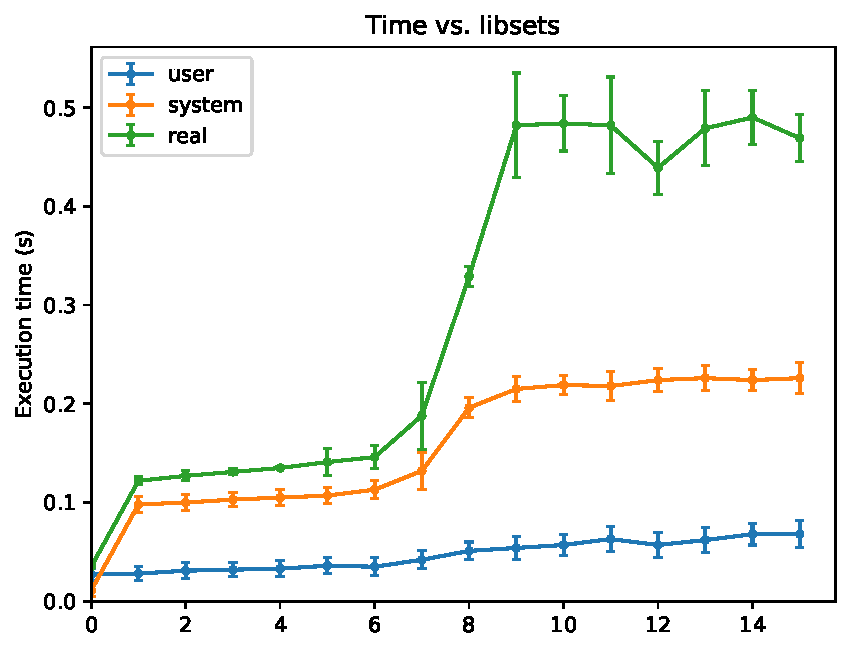
\includegraphics[width=\textwidth]{figs/dyno-baseline-times}
	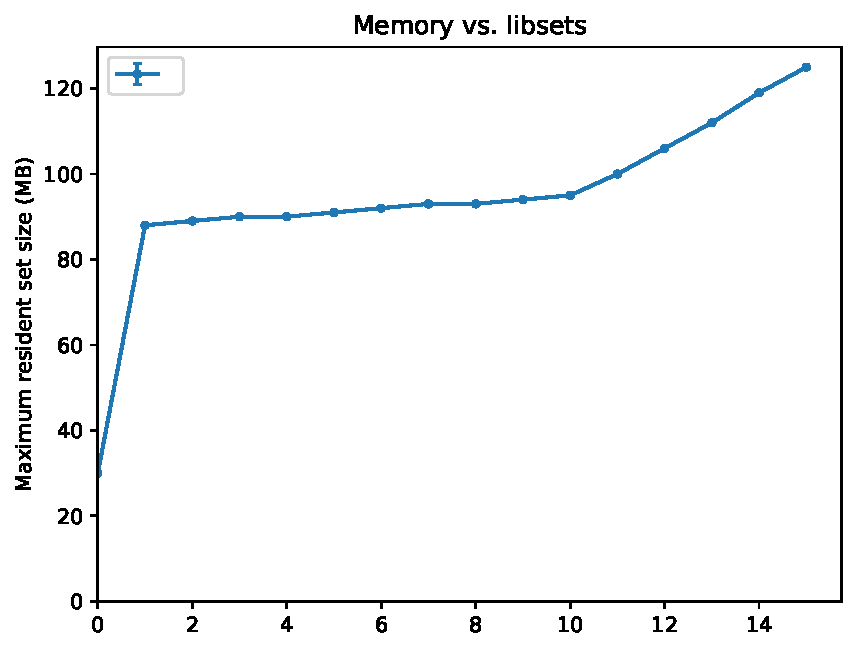
\includegraphics[width=\textwidth]{figs/dyno-baseline-memory}
	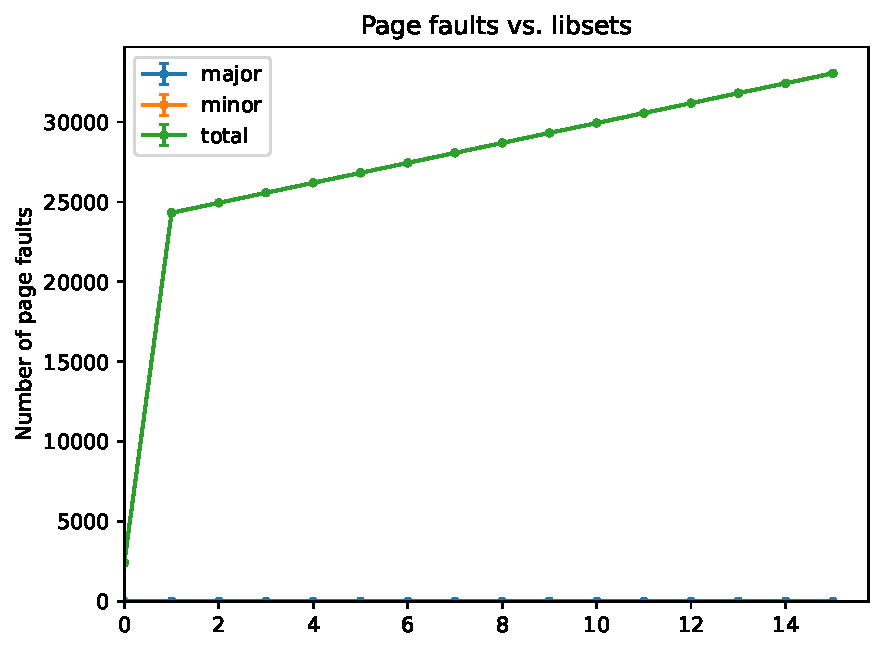
\includegraphics[width=\textwidth]{figs/dyno-baseline-faults}
	\subcaption{Deno JavaScript runtime}
	\label{fig:libgotcha:deno}
	\end{minipage}
%
	\begin{minipage}{0.5\textwidth}
	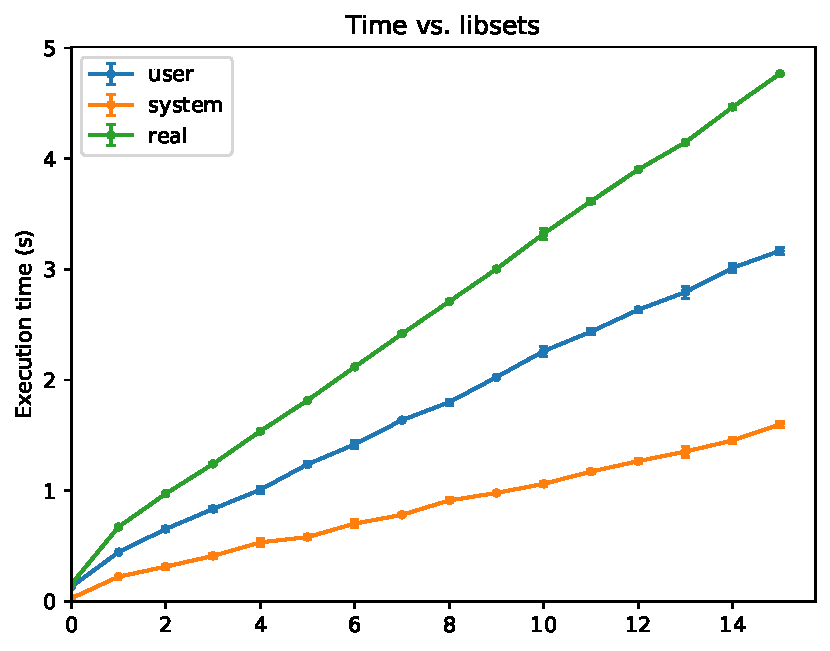
\includegraphics[width=\textwidth]{figs/dyno-times}
	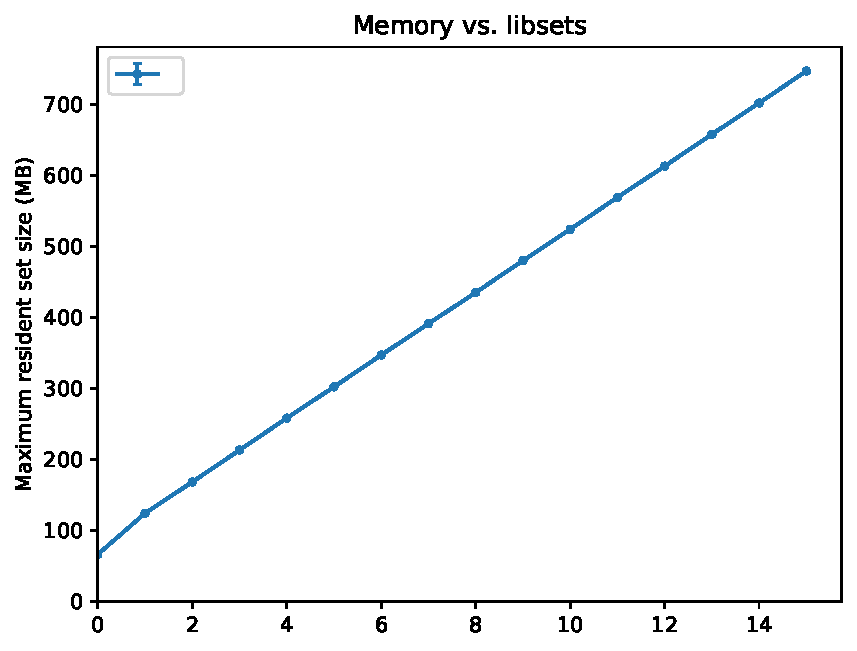
\includegraphics[width=\textwidth]{figs/dyno-memory}
	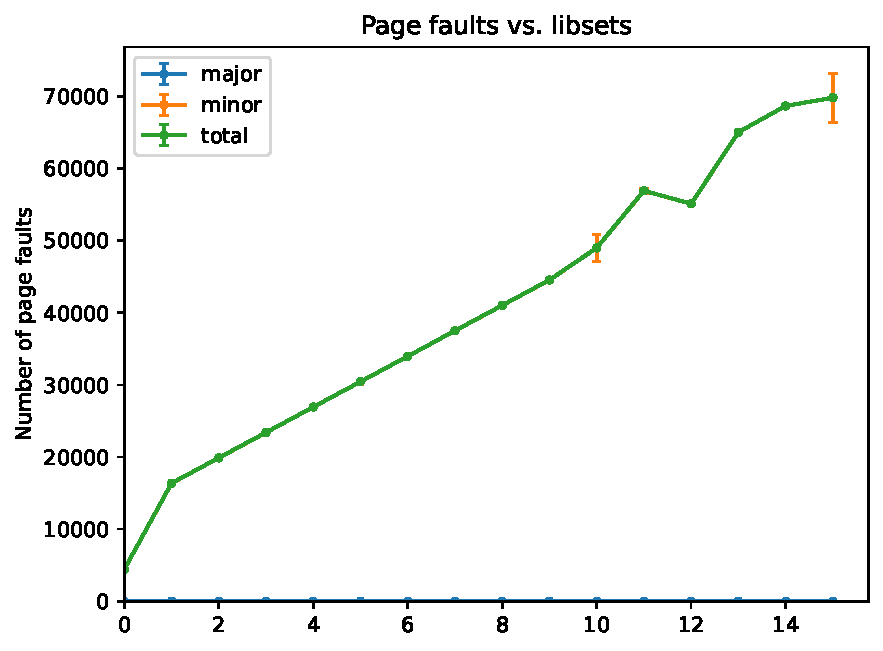
\includegraphics[width=\textwidth]{figs/dyno-faults}
	\subcaption{``Dyno'' Javascript runtime}
	\label{fig:libgotcha:dyno}
	\end{minipage}
\caption{Effect of \textit{libgotcha} on process startup}
\end{figure*}


\subsection{Thread spawn performance}
\label{sec:libgotcha:libtlsblock}

\begin{figure*}
	\begin{minipage}{0.5\textwidth}
	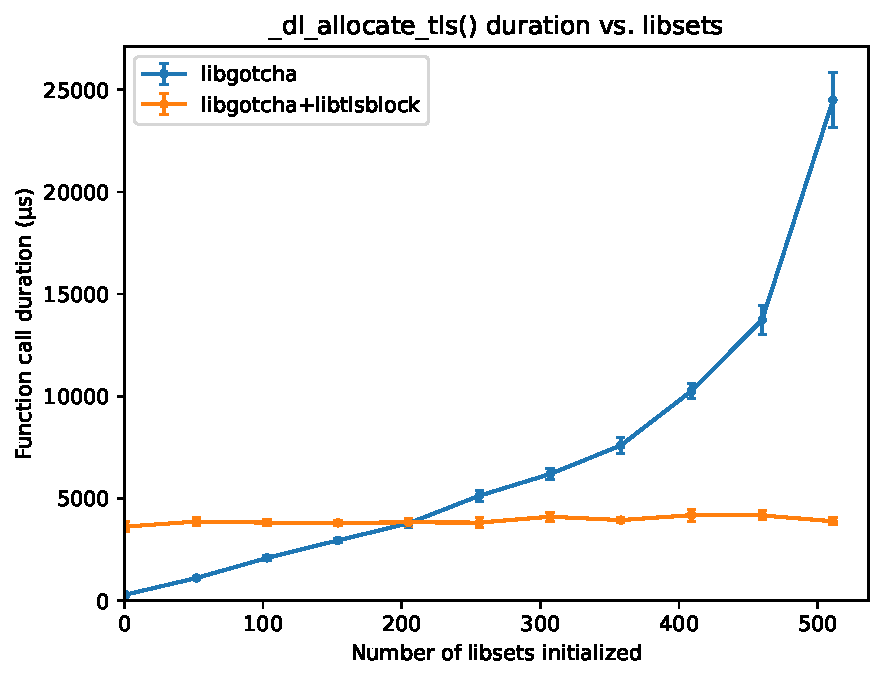
\includegraphics[width=\textwidth]{figs/tlsblock-rperfb}
	\subcaption{\texttt{\_dl\_allocate\_tls()} in isolation}
	\end{minipage}
%
	\begin{minipage}{0.5\textwidth}
	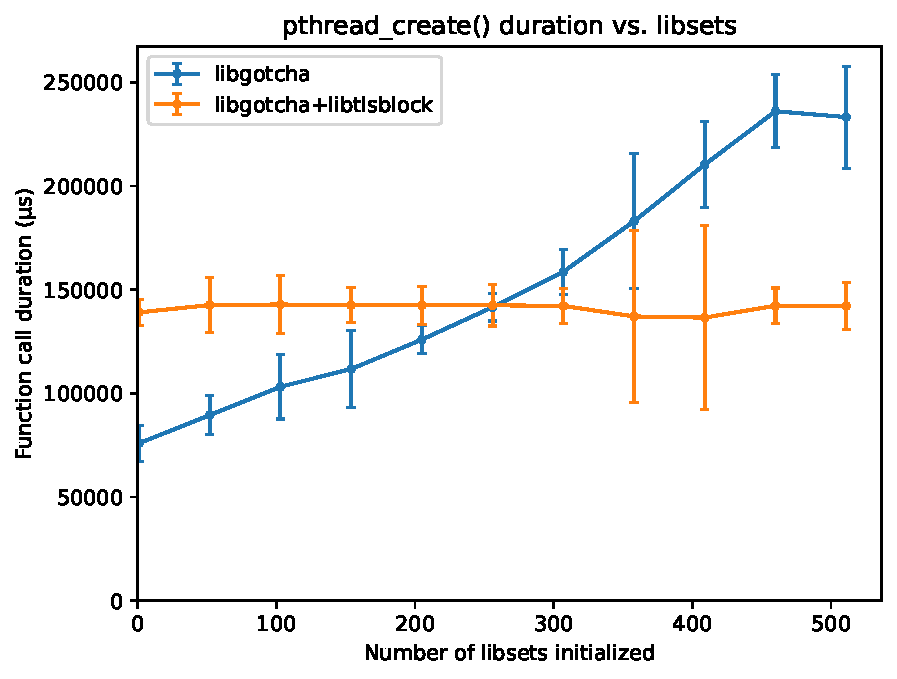
\includegraphics[width=\textwidth]{figs/tlsblock-spawn}
	\subcaption{\texttt{pthread\_create()} and \texttt{pthread\_join()}}
	\end{minipage}
\caption{Effect of \textit{libgotcha} on thread spawn latency, with and without \textit{libtlsblock}}
\label{fig:libgotcha:spawntls}
\end{figure*}

While evaluating the latency of operations under \textit{libgotcha}, we encountered a
surprising degradation in thread spawn performance.  Further investigation revealed
that the duration of each \texttt{pthread\_create()} was proportional to the number
of libsets we had initialized.  The culprit turned out to be our large static TLS
footprint (Section~\ref{sec:libgotcha:scalability}).  When allocating a TLS, glibc
iterates over each module that uses static TLS space, \texttt{memcpy()}s its
initialization image from the \texttt{.tdata} section of its module, and
\texttt{memset()}s an area the size of its \texttt{.tbss} section.  When
spawning a thread, the new TCB and TLS are merged into the \texttt{mmap()} stack
allocation to avoid having to commit heap space.  However, glibc then uses the
aforementioned initialization process on the static portion of the TLS, which
immediately faults all its pages and zeroes memory that the kernel had already
cleared.  In the case of \textit{libgotcha}, the performance impact is particularly
severe.

We hypothesized that this problem could be solved by initializing the entire TLS at
once with a single copy-on-write mapping.  To confirm this, we built a small
proof-of-concept library called \textit{libtlsblock} that interposes the
\texttt{\_dl\_allocate\_tls()} and \texttt{pthread\_create()} functions with
wrapper implementations that do exactly that.  Our finding, shown in
Figure~\ref{fig:libgotcha:spawntls}, was that this approach incurs a latency overhead
of just under 100\% for thread spawns at small numbers of
libsets, but that the cost remains flat as the number of libsets
increases, with a break-even point at about 250 libsets.  It would be easy to
tweak \textit{libtlsblock} to only activate at this number of libsets.
